\documentclass{article}
\usepackage{graphicx}
\usepackage{amsmath}
\usepackage{algorithm}
%\usepackage{algorithmic}
\usepackage{caption}


%%%%%%%%%%%%%%%%%%%%%%%%%%%%%%%%%%%%%%%%%%%%%%%%%%%%%%%%%%%%%%%%%%%%%%%%%%
% Pseudocode using algpseudocode and algorithm packages
%%%%%%%%%%%%%%%%%%%%%%%%%%%%%%%%%%%%%%%%%%%%%%%%%%%%%%%%%%%%%%%%%%%%%%%%%%

\usepackage{algpseudocode}
\usepackage{algorithm} 

\errorcontextlines\maxdimen

% begin vertical rule patch for algorithmicx (http://tex.stackexchange.com/questions/144840/vertical-loop-block-lines-in-algorithmicx-with-noend-option)
\makeatletter
% start with some helper code
% This is the vertical rule that is inserted
\newcommand*{\algrule}[1][\algorithmicindent]{\makebox[#1][l]{\hspace*{.5em}\vrule height .75\baselineskip depth .25\baselineskip}}%

\newcount\ALG@printindent@tempcnta
\def\ALG@printindent{%
    \ifnum \theALG@nested>0% is there anything to print
        \ifx\ALG@text\ALG@x@notext% is this an end group without any text?
            % do nothing
            \addvspace{-3pt}% FUDGE for cases where no text is shown, to make the rules line up
        \else
            \unskip
            % draw a rule for each indent level
            \ALG@printindent@tempcnta=1
            \loop
                \algrule[\csname ALG@ind@\the\ALG@printindent@tempcnta\endcsname]%
                \advance \ALG@printindent@tempcnta 1
            \ifnum \ALG@printindent@tempcnta<\numexpr\theALG@nested+1\relax% can't do <=, so add one to RHS and use < instead
            \repeat
        \fi
    \fi
    }%
\usepackage{etoolbox}
% the following line injects our new indent handling code in place of the default spacing
\patchcmd{\ALG@doentity}{\noindent\hskip\ALG@tlm}{\ALG@printindent}{}{\errmessage{failed to patch}}
\makeatother
% end vertical rule patch for algorithmicx


%%%%%%%%%%%%%%%%%%%%%%%%%%%%%%%%%%%%%%%%%%%%%%%%%%%%%%%%%%%%%%%%%%%%%%%%%%
%%%%%%%%%%%%%%%%%%%%%%%%%%%%%%%%%%%%%%%%%%%%%%%%%%%%%%%%%%%%%%%%%%%%%%%%%%

\begin{document}

\section{Principle of permeation counting}
\label{sec:comptage_permeation}

A permeation is the event that starts with a water membrane entering the membrane and ends with the membrane exiting into the opposite water compartment where it was previously located, see Fig.1.

\begin{figure}[ht]
    \centering
    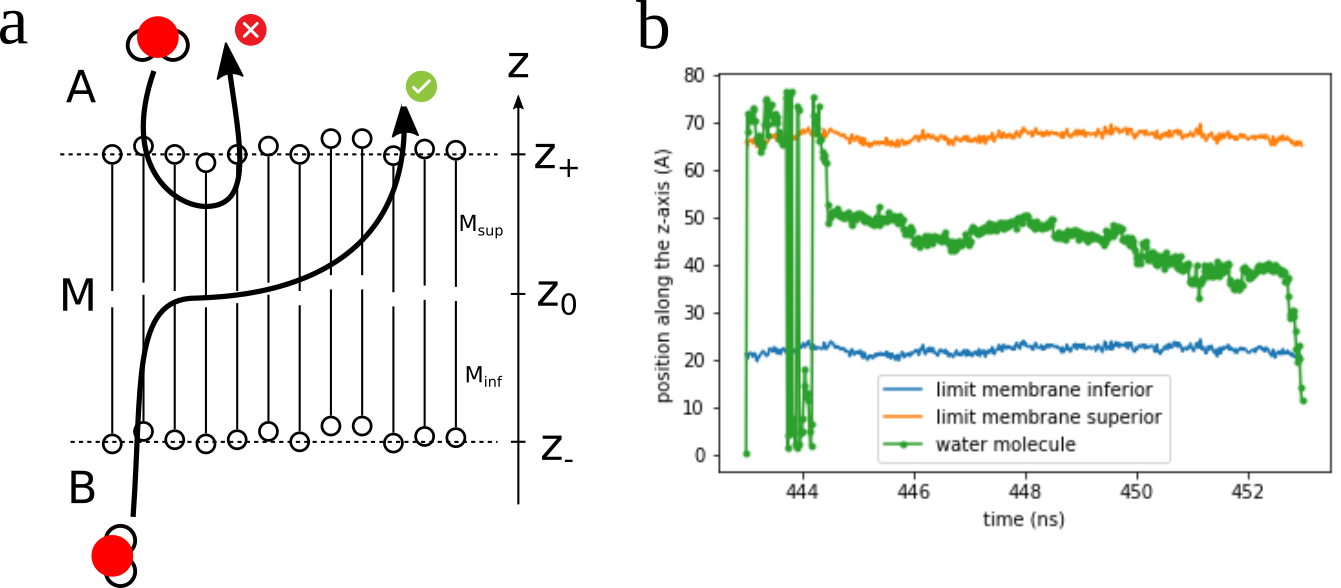
\includegraphics[width=\textwidth]{images/schema_permeation.png}
    \caption[Permeation counting]{a) Diagram of a permeation event and definition of notations. b) Trajectory of a water molecule along the $z$ direction normal to the membrane as a function of time covering the duration of a water permeation.}
    \label{schema_permeation}
\end{figure}

\section{Algorithm}
\label{sec:permeation_algorithm}


The algorithm takes place in two stages:
1) The calculation of a simplified 3-states trajectory
2) The detection of the permeation event from the simplified trajectory.

These stages are repeated for all water molecule chunks, preventing the creation of large NumPy integer arrays. If an array becomes too large due to an excessive number of timeframes, the algorithm will prompt the user to increase the number of chunks.

In the first stage, we define the state of a molecule depending on its positon along z axis. For this purpose we compute the trajectory of the lower and upper leaflets defined by the average z-coordinates over all phosphorus atoms belonging to the same leaflet ($z_+(t)$ and $z_-(t)$, see Fig.1). The state of the $i$th water molecule is defined as follows :

\begin{equation}
S^i(t) = 
    \begin{cases} 
    +1 & \text{if } z^i(t) > z_+(t) \\ 
    -1 & \text{if } z^i(t) < z_-(t) \\ 
    0 & \text{if } z_-(t) < z^i(t) < z_+(t) 
    \end{cases}
\end{equation}

Another correction is applied on the water molecules in the membrane which depends on the pre-computed displacement $\Delta z^i(t) = z^i(t) - z^i(t-\Delta t)$ of each particule. If a water molecule undergoes a large jump from or to the central membrane region ($\Delta z^i(t) > MIN\_DISP\_MEMB$ or $\Delta z^i(t+\Delta t) > MIN\_DISP\_MEMB$), then we assume this large displacement to be due to the diffusion of the water through the closest water bulk following by the periodic boundary jump. We therefore change the state $S(t)$ of the molecule according to the following criteria :

\begin{equation}
    S^i(t) \gets 
        \begin{cases} 
        +1 & \text{if } z_0(t) < z^i(t) < z_+(t) \\ 
        -1 & \text{if } z^i(t) < z_-(t) < z_0(t) \\ 
        \end{cases}
    \end{equation}

In the original implementation of the code, this criterion was introduced to prevent counting events where a water molecule crosses the periodic boundary immediately after leaving or entering the membrane. These particular cases were observed when the saving time step in the algorithm was taken large, i.e. on the order of magnitude of the average displacement of a water molecule in the bulk. However, in order to to avoid any artifacts due to the periodic boundary crossings, it is highly recommended to work with small saving time step (e.g. a good tradeoff is $\Delta t = 50 ps$). Then this correction should not be necessary. Moreover, it has been shown that for $\Delta t > 100ps$, this correction procedure introduces another bias that overestimates the real number of permeations. An example is a molecule being just above $z_0(t)$ and jumping to the lower water compartment through the membrane/channel; in this case the event after analysis of the simplified trajectory would be mistaken for permeation.

The operations performed in the first step involves NumPy arrays of size $N\times T$ where $N$ is the number of water molecules in a chunk and $T$ the number of frames.

In the second stage of the algorithm, we performed on each single water simplified trajectory $S^i(t)$ to identify the possible permeation events. First we compute an $T$-NumPy array $history^i(t)$ that stores at time $t$ the time duration that a water molecule stay in the membrane. The sign of $history^i(t)$ provides information on the last bulk region occupied by the water molecule before entering the membrane.

In order to identify a permeation event, we look for the frame $t$ for which these two conditions are met :\\
a) the water molecule has just moved from the membrane to the bulk \\
b) the sign of the jump $\Delta S^i(t) = S^i(t) - S(t - \Delta t)$ is opposite to the last bulk state visited

In this part of the algorithm, the operations are performed on $T$-NumPy arrays carrying unsigned integers.

\section{Best practices}
\label{sec:best_practices}

Although it is tempting to use a time step that is not too small to save disk memory, it is important to remember that biases can appear in the algorithm's results if the time step is too large. The user is therefore advised to always test at least once the influence of the time step on the number of events detected (e.g. 100 ps, 50 ps, 20 ps). The smaller the height of the water layer above the membrane, the greater the error, so 50 ps is not always a reliable value, depending on the geometry of your system.

\begin{algorithm}
    \caption{Compute permeations events through a lipid membrane in MD simulations}
    \begin{algorithmic}[1]
    
    \State Set \( \text{MIN\_DISP\_MEMB} \) \Comment{the minimum displacement to account for a PBC jump}
    
    \State From the phosphorus atom coordinates, compute \( T \)-arrays with:
    \State \( z^{+}[T] \): position of the upper membrane boundary
    \State \( z^{-}[T] \): position of the lower membrane boundary
    \State \( z_{0}[T] = \frac{z^{+}[T] + z^{-}[T]}{2} \): position of the center of the membrane 

    \\
    \For{all groups of water molecules} 

    \Comment{option to avoid large memory in RAM}
        \State \textbf{Compute a simplified water trajectory}
        \State \( S_{b}^{+}[T] \gets (z[T] > z^{+}[T]) \) \Comment{1 if in upper bulk region, else 0}
        \State \( S_{b}^{-}[T] \gets - (z[T] < z^{-}[T]) \) \Comment{-1 if in lower bulk region,else 0}
        \State \( S_{m}^{+}[T] \gets \text{1 if in upper membrane region, else 0} \)
        \State \( S_{m}^{-}[T] \gets \text{-1 if in lower membrane region, else 0} \)
        \State \( S_{\text{jump}}[T] \gets \text{array with 1 if jump with } |dz| > \text{MIN\_DISP\_MEMB} \)
        \State \( S[T] \gets S_{b}^{-}[T] + S_{b}^{+}[T] + (S_{m}^{-}[T] + S_{m}^{+}[T]) \cdot S_{\text{jump}}[0:T-1] + (S_{m}^{-}[T] + S_{m}^{+}[T]) \cdot S_{\text{jump}}[1:T] \)

        \Comment{simplified 3-state trajectory with corrections from close bulk state if involved in a PBC jump}
        \\

        \For{all \( N \) water molecules}
            \State \textbf{Compute the history of a single molecule}
            \State \( \text{history} \gets 0 \) \Comment{to store history state and time}
            \State \( \text{memory} \gets 0 \) \Comment{intermediary variable}
            
            \For{t over T frames}
            \State \( \text{history}[t] \gets S[t] \)
            \If{$S[t] = 0$} \Comment{the water molecule is in the membrane}
                \State \( \text{history}[t] \gets \text{memory} + \text{sign}(\text{memory}) \) \Comment{cumulate history}
            \EndIf
            \State \( \text{memory} \gets \text{history}[t] \)
        \EndFor
            
            \State \textbf{Compute state variation}
            \State \( \Delta S[T] \gets S[1:T] - S[0:T-1] \)
    
            \State \textbf{Detect permeation events}

            \State \( \text{events}[T] \gets \) \Comment{A permeation event occurs when :}
            \State \( \Delta S[T] \) \Comment{ the water molecule cross a region boundary}
            \State \( \cdot (S[T] - \Delta S[T] == 0) \) \Comment{the molecule goes from membrane to bulk}
            \State \(\cdot (\Delta S[T] \cdot (\text{history}[T])< 0) \) \Comment{the direction of movement points towards the opposite of the last visited bulk region}
    
            \For{t over T frames}
                \If{$events[t] \neq 0$} \Comment{permeation event detected}
                    \State Store molecule id \( i \)
                    \State Store permeation time \( t \)
                    \State Store permeation duration \( |\text{history}[t]| \)
                    \State Store permeation direction \( \text{diff}[t] \)
                \EndIf
            \EndFor
        \EndFor
    \EndFor
    
    \end{algorithmic}
\end{algorithm}

\end{document}
